\newpage
\chapter{NEPALI HANDWRITTEN DATASETS}\label{chapter_nepali_handwritten_database}

To do experimentation with this research work, benchmark datasets for Off-line Nepali Handwritten Characters are created. There are three separate datasets for Nepali handwritten consonants, vowels and numerals. The overall dataset creation procedure is discussed in section \ref{section_dataset_creation_procedure}. More detail about Nepali consonant dataset, vowel dataset and numeral dataset is given in the section \ref{section_consonant_dataset}, section \ref{section_vowel_dataset} and section \ref{section_numeral_dataset}, respectively. Training and testing samples for recognition system are selected from each dataset in certain ratio.

\section{Dataset Creation Procedure}\label{section_dataset_creation_procedure}
Datasets are created by taking handwriting samples from different writers from different fields. The overall procedure for creating off-line Nepali handwritten character datasets is described in the Algorithm \ref{algorithm_dataset_creation}.

\begin{algorithm}
\caption{Handwritten Dataset Creation}
\label{algorithm_dataset_creation}
\begin{algorithmic}[1]
\STATE  Take handwritten samples from different writers in A4 paper.
\STATE  Scan the sample documents using digital scanner.
\STATE  Slice and crop individual characters from each documents.
\STATE  Make individual directory for each category of datasets.
\STATE	Make individual class directory in each dataset directory.
\STATE  Drag individual characters in the corresponding class directory.
\STATE  Datasets are ready.
\end{algorithmic}
\end{algorithm}

\pagebreak
\section{Nepali Handwritten Consonant Dataset}
\label{section_consonant_dataset}

Nepali language contains $36$ different Devanagari alphabets for Consonants. Figure \ref{figure_ka_kha} shows Nepali handwritten consonants. To create training and testing dataset of Nepali handwritten consonants, handwritten consonant images are scanned with digital scanner and cropped for individual characters.

Nepali handwritten consonant dataset contains total $\textbf{7380}$ image samples. Samples are taken from $45$ different writers from different fields. Each class of consonant dataset contains $205$ images with varying styles and shapes.
\begin{figure}[h]
\centering
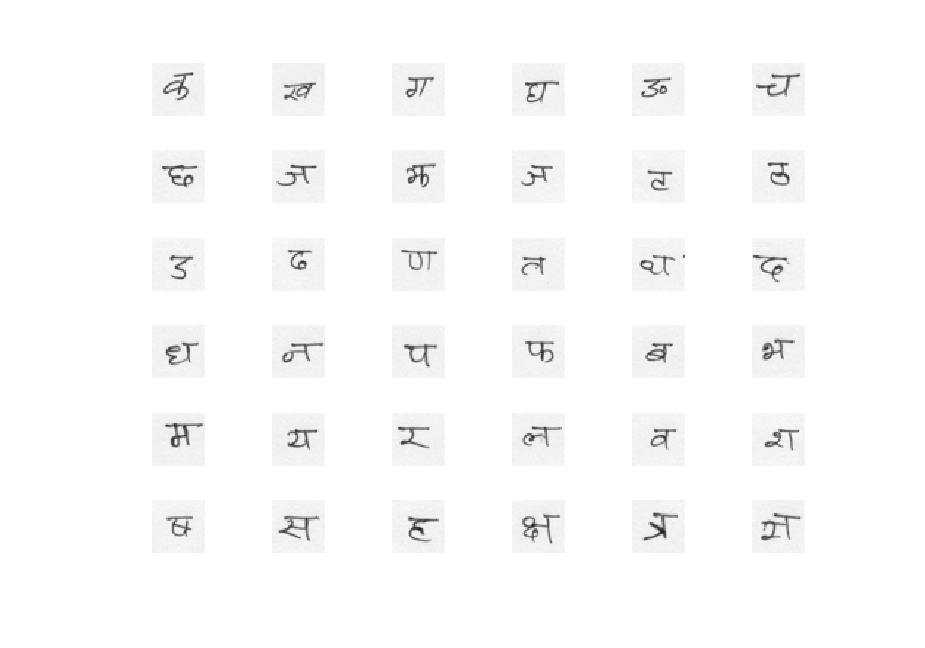
\includegraphics[width=4in]{figures/datasets/nhcr/ka_kha_sample.eps}
\caption{Nepali Handwritten Consonants.}
\label{figure_ka_kha}
\end{figure}

\section{Nepali Handwritten Vowel Dataset}
\label{section_vowel_dataset}
Nepali language contains $12$ different Devanagari alphabets for vowels. Figure \ref{figure_a_aa} shows Nepali handwritten vowels. To create training and testing dataset of Nepali handwritten vowels, handwritten vowel samples are scanned with digital scanner and cropped for individual characters.

Nepali handwritten vowel dataset contains total $\textbf{2652}$ image samples. Samples are taken from $44$ different writers from different fields. Each class of vowel dataset contains $221$ images with varying styles and shapes.
\begin{figure}[h]
\centering
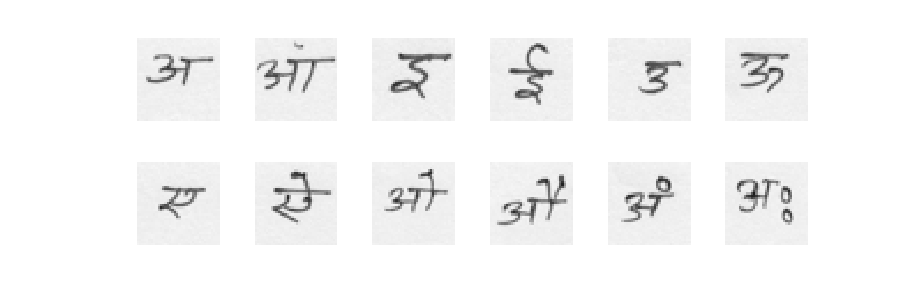
\includegraphics[width=4in]{figures/datasets/nhcr/a_aa_sample.eps}
\caption{Nepali Handwritten Vowels.}
\label{figure_a_aa}
\end{figure}

\section{Nepali Handwritten Numeral Dataset}
\label{section_numeral_dataset}

Nepali language contains $10$ different Devanagari numerals. Figure \ref{figure_one_two} shows Nepali handwritten numerals. To create training and testing dataset of Nepali handwritten numerals, handwritten numeral images are scanned with digital scanner and cropped for individual characters.

Nepali handwritten numeral dataset contains total $\textbf{2880}$ image samples. Samples are taken from $45$ different writers from different fields. Each class of numeral dataset contains $288$ images with varying styles and shapes.
\begin{figure}[h]
\centering
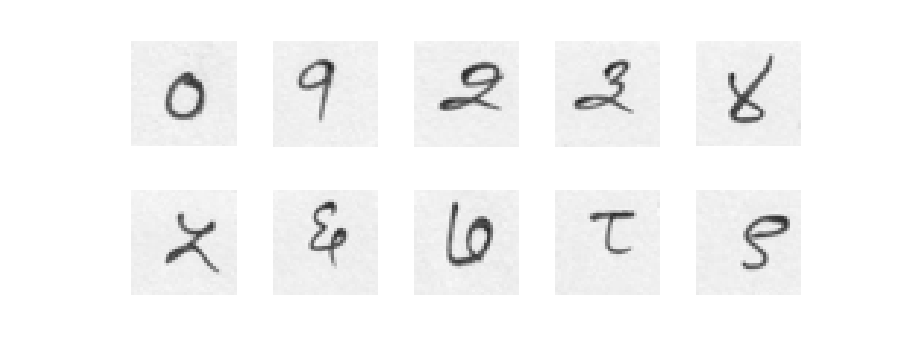
\includegraphics[width=3in]{figures/datasets/nhcr/one_two_sample.eps}
\caption{Nepali Handwritten Numerals.}
\label{figure_one_two}
\end{figure}